\chapter{Voltage unbalance indication}\label{BASIC:sec:main}

In this chapter the basic topics of the thesis are discussed, as components for further understanding. First the phenomena of voltage unbalance on small distribution networks are shown and the ambiguities though the development of the concept, and at the end the norm currently being in use in the industry. It would be shown how many definitions are currently in use, thus the introduced ambiguity of definition, further validating the proposal in section \ref{VUB:sec:Geom}.\\
After the introduction the proposed geometrical indicator and control cost-function candidate, shall be discussed and compared against the standardised method, the voltage unbalance factor, $VUF$ via correlation investigation.
%Next a necessary glimpse of power electric background is given to invite to the viewpoint of the modeling and problem breakdown of power converter. The section would introduce the background of current source switching devices with forced commutation, since control based on external situations or according to a cost function is eminent. After the single phase method shall be described, DC-DC conversion would be shown, since in section \ref{VUB:sec:Compensation} non-zero mean asymmetrical power injection was required. The section closes with the three phase rectifier example, for contributing the understating of the modeling in section \ref{EMPC:sec:Modeling}.\\
%Further the basis of controller structures, shall be shown, applied in the thesis. These are the APPS (asynchronous parallel pattern search) method (used in section \ref{VUB:sec:Optimization}) and constrained model based predictive control (MPC) is to be described with the end with the explicit partition of the state space (explicit MPC applied in section \ref{EMPC:sec:DCside}) for a computationally efficient approach.\\
%Lastly a new approach shall be discussed around the phenomena of voltage unbalance in a small domestic network. First the networks structure shall be described, the power electrical system is connected to, as a household supplying, renewable utilizing device. Then a control cost-function candidate, the proposed geometrical approach shall be presented, as an indicator of voltage unbalance.

\section{Literature overview}

%============ RENEWABLE SYSTEM
Single phase power injections to the grid are mainly generated by domestic photovoltaic-(PV) and wind power plants. For off-grid, sometimes more complex solutions integrating diesel generators, PV and wind generators. Such as proposed, in \cite{shezan2016}, and \cite{cucchiella2013environmental}, where presented the economical aspects of a PV system. The economic results are strongly influenced by the annual average isolation value, which encourages the areas most exposed to the sun and the southern areas. The consumption of consumers is not critically important, but the design principle used has as significant effect on the maximization of the performance of PV plants. In the paper \cite{kaldellis2009optimum} it is worth noticing, that autonomous photovoltaic systems are strongly responsible of their reactive energy requirements. To support photovoltaic systems with sufficient battery banks one should be able to establish that their reactive energy requirement share fairly compensated by the corresponding energy yield.  Additionally, in \cite{ortega2013measurement} the author emphasizes that PV systems are increasingly being deployed in all over the world, and this is the source of a wide range of power quality problems. With a view on consistently measuring and assessing the power quality characteristics of PV systems, they had presented an in-depth overview and discussion of this topic.\\
%============ EV SYSTEM
 The study \cite{huat2015integration} explored implementation issues of electric vehicle battery packs. They suggest that high voltage battery packs with large format cells has advantages in assembly, thermal management, monitoring and control, services and maintenance. On the other hand, quality, reliability and limited specific energy of large format cells are obstacles need to overcome. Solving these problems will further affect the cost, performance, reliability and safety of the electric vehicles. Smart energy systems in specially in urban areas are discussed in \cite{lund2015smart} where a design methodology has been suggested.\\
%============ EFFECTS OF UNBALANCE
Many power systems, voltage parameters change over time. Variation of power quality leads to thermal transients in electrical machines. This problem can be especially important in the case of low-power machines, because they have shorter time constants than high-power ones. The rate of thermal responses of a machine also significantly depends on the type of power quality disturbances. Voltage unbalance can cause  machine  overheating  within  a  mere  few  minutes. Furthermore,  fluctuating  unbalance  could  cause  an  extraordinary rise  in  windings  temperature  and  additional  thermo-mechanical stress.  Consequently,  voltage  unbalance  is  found  to  be  more harmful to induction motors than the results from previous work \cite{gnacinski2019induction}. Additionally beside the heat factor, voltage unbalance can cause increased reactive power \cite{savaghebi2012secondary}, various copper loss \cite{siddique2004effects} torque pulsation in electric motors \cite{brekken2005control}. The authors of \cite{lee1998effects} were discussing the effects of unbalanced voltage on a three-phase induction motor, one has to consider not only negative-sequence voltage but also the positive-sequence voltage. With the same voltage unbalance factor, the status of voltage unbalance could be judged by the magnitude of positive sequence voltage. Also the effect of voltage unbalance has been studied on three-phase four-wire distribution networks for different control strategies for three-phase inverter-connected distributed generation units on voltage unbalance in distribution networks \cite{meersman2011three}. Here the negative-sequence component and the zero sequence component were studied where unbalance conditions could lower stability margin and increasing the power losses. On the other hand, the adaptive coordination of distribution systems included distributed generation is also an emerging problem as it was discussed by \cite{ates2016}.  A small voltage unbalance might lead to a significant current unbalance because of low negative sequence impedance as highlighted in \cite{bina2011three}.\\
%============ DEPARTMENT WORK REGARDING UNBALANCE
As such a previous work of \cite{gorbe2012reduction} a complex control unit has been proposed that is capable of lowering extant harmonic distortion. In the work of \cite{Gorbe2014experimental} the effect of a small domestic (photovoltaic) power plant on the power quality, mainly the total harmonic distortion has been examined. The aim of this work is to examine and compensate three phase voltage asymmetry of the electrical network based on the extended simulation model proposed by \cite{gorbe2012reduction}. Further control methods were applied for the solution for balancing of the most sensitive with regard to electric energy quality part of power system in \cite{korovkin2016uimethod},  minimizing the active power losses, stabilization of three-phase voltages, enhancement of asynchronous machine performance stability and reduction of errors occurring in power consumption measuring circuits.\\
%============ UNBALANCE CALCULATION
In many articles the authors presents a different viewpoint of calculating unbalance on the network. \cite{martin2015unbalance} showed to assess the harmonic distortion and the unbalance introduced by the different loads connected to the same point of common coupling have been applied to an experimental distribution network.  By \cite{kini2007novel} the focus was to bring out the ambiguity that crops up when we refer to a particular value of voltage unbalance that exists in the system. By making use of the complex nature of voltage unbalance, the voltage combinations that lead to the calculation of complex voltage unbalance factor could be narrowed down to a great extent. A fast and accurate algorithm for calculating unbalance has been presented by \cite{wen2014approximate}. The magnitudes of zero, positive, and negative sequences are obtained through simple algebraic equations based on the geometric figure, which is also called as 4 and 8 geometric partitions. Also a three-phase optimal power flow calculation methodology has been presented by \cite{araujo2013three}, that is suitable for unbalanced power systems. The optimal algorithm uses the primal-dual interior point method as an optimization tool in association with the three-phase current injection method in rectangular coordinates.\\

\section{Definitions of voltage unbalance}\label{BASICUNB:sec:DefinitionsofUNB}

%\textbf{(Mostly) from Wikipedia:}\\
In a symmetric three-phase power supply system, three conductors each carry an alternating current of the same frequency and voltage amplitude relative to a common reference but with a phase difference of one third of a cycle between each. The common reference is usually connected to ground and often to a current-carrying conductor called the neutral. Due to the phase difference, the voltage on any conductor reaches its peak at one third of a cycle after one of the other conductors and one third of a cycle before the remaining conductor. This phase delay gives constant power transfer to a balanced linear load.\\
In general symmetric three-phase systems described, are simply referred to as three-phase systems because, although it is possible to design and implement asymmetric three-phase power systems (i.e., with unequal voltages or phase shifts), they are not used in practice because they lack the most important advantages of symmetric systems. In a three-phase system feeding a balanced and linear load, the sum of the instantaneous currents of the three conductors is zero. In other words, the current in each conductor is equal in magnitude to the sum of the currents in the other two, but with the opposite sign. The return path for the current in any phase conductor is the other two phase conductors.\\
Constant power transfer and cancelling phase currents would in theory be possible with any number (greater than one) of phases, maintaining the capacity-to-conductor material ratio that is twice that of single-phase power. However, two-phase power results in a less smooth (pulsating) torque in a generator or motor (making smooth power transfer a challenge), and more than three phases complicates infrastructure unnecessarily.\\
Three-phase systems may also have a fourth wire, particularly in low-voltage distribution. This is the neutral wire. The neutral allows three separate single-phase supplies to be provided at a constant voltage and is commonly used for supplying groups of domestic properties which are each single-phase loads. The connections are arranged so that, as far as possible in each group, equal power is drawn from each phase. Further up the distribution system, the currents are usually well balanced. Transformers may be wired in a way that they have a four-wire secondary but a three-wire primary while allowing unbalanced loads and the associated secondary-side neutral currents \cite{von2006electric}.

\subsection{Phenomena of voltage unbalance}\label{BASICUNB:sec:PhenomenafUNB}

In a domestic network, three-phase electric power systems have at least three conductors carrying alternating voltages that are offset in time by one-third of the period. A three-phase system may be arranged in delta  or star. A star system allows the use of two different voltages from all three phases, such as a 230/400 V system which provides 230 V between the neutral (center hub) and any one of the phases, and 400 V across any two phases displayed on Fig.\ref{BASICUNB:fig:UnbWave}. The definition is the following:
	
			\begin{equation}
        \begin{array}{rcl}
            \vec{V}_a&=&\hat{V}\,sin(\theta)\\
						\vec{V}_b&=&\hat{V}\,sin(\theta+\frac{4}{3}\pi)\\
						\vec{V}_c&=&\hat{V}\,sin(\theta+\frac{2}{3}\pi),\\
        \end{array}
        \label{BASICUNB:equ:Definition}
    \end{equation}
	
	where $\vec{V}_a,\,\vec{V}_b,\,\vec{V}_c$ are the phase voltage vectors, $\hat{V}$ is the voltage peak, and $\theta$ is the phase angle. Voltage unbalance a phenomena where the three phase voltages differ in amplitude normal 120 degree phase relationship shown in Fig.\ref{BASICUNB:fig:UnbPhasor}. In most cases both are happening at the same time. This includes unequal voltage magnitudes at the fundamental frequency, either under, or over voltage, at the fundamental phase angle deviation.
	
	\begin{figure}[h!]
     \centering
		\begin{subfigure}[b]{0.49\textwidth}
         \centering
         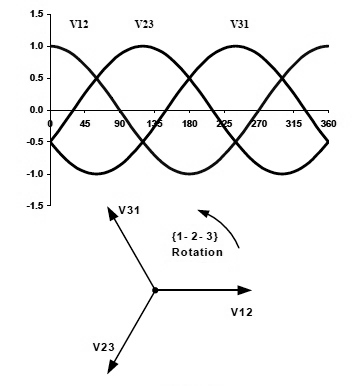
\includegraphics[width=\textwidth]{Unblance_EPS_Pics/Three-phase-voltage-system_gray.png}
         \caption{Three phase sine wave of network voltage.}
         \label{BASICUNB:fig:UnbWave}
     \end{subfigure}
		\hfill
     \begin{subfigure}[b]{0.49\textwidth}
         \centering
         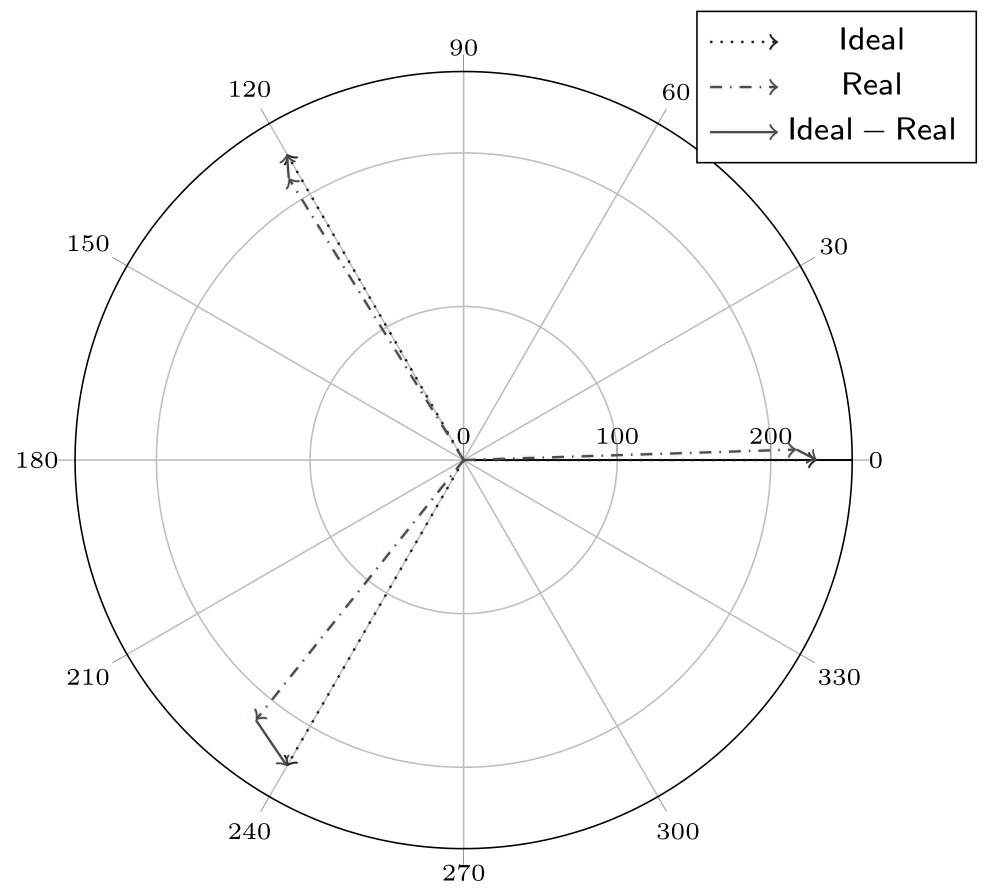
\includegraphics[width=\textwidth]{Unblance_EPS_Pics/PhasorGrayscale.jpg}
         \caption{The three phase voltage phasor whith $Ideal$ and $Real$ voltage vectors.}
         \label{BASICUNB:fig:UnbPhasor}
     \end{subfigure}
        %\caption{BASICUNB:fig:UnbPhasor}
        \label{BASICUNB:fig:UnbPhasor_all}
\end{figure}
	
	This is observed as a frequently cited power quality issue in low-voltage domestic distribution networks and in systems that supply large single phase loads distributed unevenly among the phases. Effects of voltage unbalance are complex, but can be categorized as structural or functional. The former refers to the asymmetry in the three-phase impedances of transmission lines, cables, transformers, etc. It occurs because it is neither economical nor necessary to maintain distribution system with perfectly symmetrical impedances. The latter refers to uneven distribution of power consumption over the three phases. Although the term voltage unbalance is unambiguous, the root phenomenon may be various as well as the standard norms used to measure unbalance. All of these different indicators measure voltage unbalance but each of them does it in a different way. In this section a detailed explanation is presented about the types of currently used method for indication.
	
	\subsection{Types of voltage deviations and norms}\label{BASICUNB:sec:DefinitionsofUNB}

        Voltage unbalance is not a straightforward term. To understand the concept, unbalance is when on a given frequency (mostly fundamental frequency) voltage vectors (phase or line depending on the definition) deviating from the ideal in terms of length or angle. The first fall in to the category of unbalance, namely any kind of phase deviations, and unbalanced amplitude deviations, and balanced amplitude deviations, like under-voltage. There are many different technological causes with more or less practical importance. The following conditions are examined and tested in the sequel:
        \begin{description}
        \item[Single phase under-voltage unbalance]  If there is a single phase uncompensated overload in the system, the voltage in the overloaded phase will be lower than the other two.
        \item[Two phase under-voltage unbalance]  Two of the three phases are overloaded without compensation, the two overloaded phases will have higher voltage drop than the third phase.
        Balanced three phase under-voltage]  The loads of all three phases are overloaded in an unbalanced manner.
        \item[Unbalanced single phase angle]  If the three phase voltage amplitudes are balanced but the relative angles between them (ideally it should be equal to $\pm120$ degree). It is assumed, that $V_a$ would be the reference. If one of the other two phase angles is deflected, unequal displacement.
        \item[Unbalanced two phase angles displacement] Similar to the single phase angle unbalance, if the other two phase angles are both deflected, then unequal angle displacement in two phase angles occurs.
        \end{description}
        An indicator of the voltage unbalance is supposed to measure the extent of unbalance but it is not expected to classify between the above types.
	
	\subsection{Non standardized approximation formulas}\label{BASICUNB:sec:ApproxFormula}
	
	Up to now, the following definitions have not been adopted by any standard or rule to indicate the degree of voltage unbalance, but used by various manufacturers. Firstly based on \cite{eugene1986new} recommended by the CIGRE (International Council on Large Electric Systems, in French: Conseil International des Grands Réseaux Électriques), the voltage unbalance is determined with:
	
	\begin{equation}
        \begin{array}{rcl}
            VUFactor&=&\frac{\sqrt{{1-\sqrt{3-6\frac{V_{ab}^4+V_{bc}^4+V_{ca}^4}{\left(V_{ab}^2+V_{bc}^2+V_{ca}^2\right)^2}}}}}{1+\sqrt{3-6\frac{V_{ab}^4+V_{bc}^4+V_{ca}^4}{\left(V_{ab}^2+V_{bc}^2+V_{ca}^2\right)^2}}}\\
						%\textnormal{where},&&\\
						%\upsilon&=&\frac{V_{ab}^4+V_{bc}^4+V_{ca}^4}{\left(V_{ab}^2+V_{bc}^2+V_{ca}^2\right)^2},					
        \end{array}
        \label{BASICUNB:equ:CIRGE}
    \end{equation}
		
		where, $\{V_{ab},V_{bc},V_{ca}\}$ are the line-to-line voltages. Note, that the CIRGE variant has no distinct notation, as such it would be indicated as $VUFactor$ in this thesis. Moreover, the author of \cite{robert1992assessing} recommends two more variants, based on manufacturer recommended"standards":
		
		\begin{equation}
        \begin{array}{rcl}
            VU&=&\frac{82\cdot\sqrt{(V_{ab}-V_{avg_{line}})^2+(V_{bc}-V_{avg_{line}})^2+(V_{ca}-V_{avg_{line}})^2}}{V_{avg_{line}}}\times100\\					
        \end{array}
        \label{BASICUNB:equ:VU}
    \end{equation}
		
		\begin{equation}
        \begin{array}{rcl}
            VUR&=&\frac{max\left( |V_{ab}-V_{bc}|,|V_{bc}-V_{ca}|,|V_{ca}-V_{ab}| \right)}{V_{avg_{line}}}\times100,\\				
        \end{array}
        \label{BASICUNB:equ:VUR}
    \end{equation}
		
		where the mean of line voltages is noted by $V_{avg_{line}}=\frac{V_{ab}+V_{bc}+V_{ca}}{3}$.
		This formulas were created with the intention to avoid the use of the complex algebra in symmetrical components and give
a good approximation of the later described $VUF$ standard. With the indicator of \ref{BASICUNB:equ:VU}, and as well as \ref{BASICUNB:equ:VUR}. It is worth noticing, that only the voltage magnitude unbalance is reflected, completely ignoring Fortescue's method of symmetrical components \cite{fortescue1918method} (shall presented later in the thesis), which considers negative sequence components as harmful on electric equipment and yield. Later it will be shown that other methods try to push the same methodology, until the currently used norm ($VUF$) is used.

	
	\subsection{LVUR}\label{BASICUNB:sec:LVUR}
	
	One of the first voltage unbalance in percent is defined by the National Electrical Manufacturers Association (NEMA) \cite{bonnett1997understanding} is defined  as the ratio of the maximum voltage deviation from the average line voltage magnitude to the average line-voltage magnitude.
	
\begin{equation}
        \begin{array}{rcl}
            LVUR&=&\frac{\max\left( |V_{ab}-V_{avg_{line}}|,|V_{bc}-V_{avg_{line}}|,|V_{ca}-V_{avg_{line}}| \right)}{V_{avg_{line}}}\times100\\			
        \end{array}
        \label{BASICUNB:equ:LVUR}
    \end{equation}
		
		The LVUR assumes that the average voltage is always equal to the rated value, which is 480 volts for the US three-phase systems, and it works only with magnitudes. Phase angles are not considered in this definition.
	
	\subsection{PVUR}\label{BASICUNB:sec:PVUR}
	
	The next phase voltage unbalance in percent described in IEEE standard $141.$ \cite{IEEE_141_35071} (derived from \cite{IEEE_112_8635630}), is $PVUR_{IEEE-141}$. It is defined as the ratio of the maximum voltage deviation of phase voltages from the average phase-voltage magnitude to the average phase voltage magnitude. In various fields, LVUR and $PVUR_{IEEE-141}$ are commonly used to estimate the degree of voltage unbalance due to simplicity of calculation. The two unbalance factors mentioned above cannot completely reflect system voltage unbalance effects, such as the phase displacements of unbalanced voltages.
	
	\begin{equation}
        \begin{array}{rcl}
            PVUR_{IEEE-141}&=&\frac{\max\left( |V_{a}-V_{avg_{phase}}|,|V_{b}-V_{avg_{phase}}|,|V_{c}-V_{avg_{phase}}| \right)}{V_{avg_{phase}}}\times100,\\
        \end{array}
        \label{BASICUNB:equ:PVUR-141}
    \end{equation}

where the voltages $\{V_{a},V_{b},V_{c}\}$ denotes the phase-to-neutral voltages, and $V_{avg_{phase}}=\frac{V_{a}+V_{b}+V_{c}}{3}$.
The second variant is, $PVUR_{IEEE-936}$, mentioned in \cite{IEEE_936_29053} is defined as the ratio of the difference between the highest and the lowest phase-voltage magnitude to the average phase-voltage magnitude. Therefore, the numerical values of voltage balance quantified by $PVUR_{IEEE-936}$ are generally larger than those of $PVUR_{IEEE-141}$ and LVUR.

\begin{equation}
        \begin{array}{rcl}
            PVUR_{IEEE-936}&=&\frac{\max\left( |V_a|,|V_b|,|V_c| \right)-min\left( |V_a|,|V_b|,|V_c| \right)}{V_{avg_{phase}}}\times100,\\					
        \end{array}
        \label{BASICUNB:equ:PVUR-936}
    \end{equation}
		
The number of possible combinations of three phase or line voltages that satisfy the definitions of voltage unbalance mentioned above will become infinite as only the magnitudes of voltages are considered.	
		
	
	\subsection{VUF and CVUF}\label{BASICUNB:sec:VUFCVUF}
	
	The voltage unbalance factor ($VUF$) was defined by the International Electrotechnical Commission \cite{pillay2001definitions}, \cite{dugan1996electrical}. From the theorem of symmetrical components \cite{fortescue1918method}, voltage unbalance can be considered as a phenomenon that positive sequence voltage  ($V_p$) is disturbed by negative  ($V_n$) and zero-sequence ($V_0$) voltages:
	
	\begin{equation}
        \begin{array}{rcl}
            \begin{bmatrix}
						V_0\\
						V_p\\
						V_n\\
						\end{bmatrix}&=&
						\frac{1}{3}\begin{bmatrix}
						1&1&1\\
						1&\upsilon&\upsilon^2\\
						1&\upsilon^2&\upsilon\\
						\end{bmatrix}\cdot
						\begin{bmatrix}
						V_a\\
						V_b\\
						V_c\\
						\end{bmatrix},\\
        \end{array}
        \label{BASICUNB:equ:symmetry}
    \end{equation}
	
	Where $\upsilon=e^{2j\pi/3}$ is the Fortesque operator. From that the formula of $VUF$ can be expressed as:
	
	
	\begin{equation}
        \begin{array}{rcl}
            VUF&=&\left|\frac{V_n}{V_p}\right|\times100,\\					
        \end{array}
        \label{BASICUNB:equ:VUF}
    \end{equation}

    \begin{figure}[h]
         \centering
         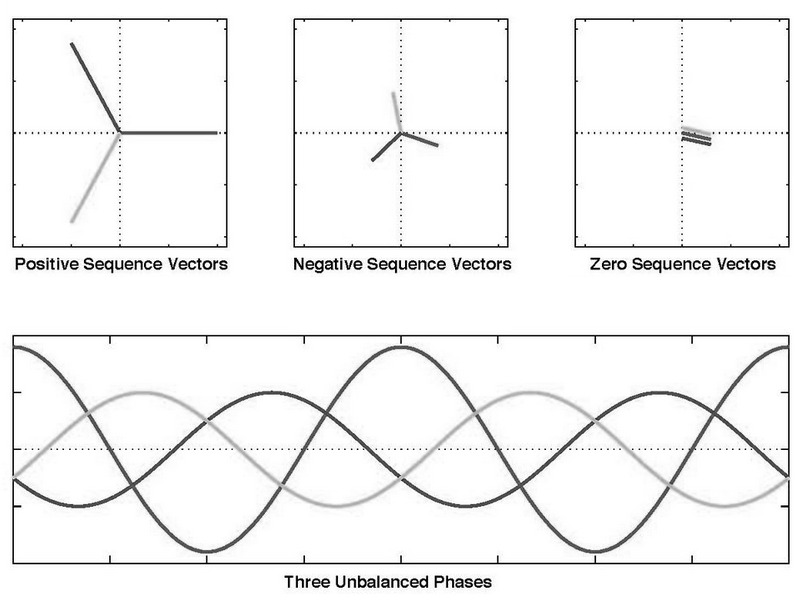
\includegraphics[width=.7\textwidth]{Unblance_EPS_Pics/Symmetrical_components_gray.jpg}
         \caption{Simplified graphical display of symmetrical components.}
         \label{BASICUNB:fig:symmetrical_simple}
     \end{figure}
	
This norm is currently in use world wide for voltage unbalance indication. The main focus in on the negative sequence component $V_n$, on which many studies attributes importance of the cause of negative effects the voltage unbalance causes.\\
	As such, three-phase electric loads without path through the neutral, negative-sequence voltage is the primary cause of voltage unbalance. Normally, positive-sequence component of three-phase voltages is very close to rated value. If expressed in per-unit quantities, the positive-sequence voltage will be very close to $1.0$ p.u., and the corresponding negative-sequence voltage will be very close to the $VUF$. Thus, the $VUF$ can indeed be considered as the negative-sequence component in per-unit.	This explains the advantage of using the VUF as an index for analyzing the effects of voltage unbalance considering the phase deviations.
	An extension of the VUF is the complex voltage unbalance factor ($CVUF$) that is defined by the ratio of the negative-
sequence voltage phasor to the positive-sequence voltage phasor studied in \cite{wang2000analytical}, and \cite{pierrat1987unbalance}. The CVUF is a complex quantity having the magnitude and the angle. Although the CVUF has not yet been widely used by practicing engineers, it has been proposed in some studies (e.g., \cite{wang2001analysis}, \cite{singh2007some}, \cite{chen2013examination}) due to its richness of information on unbalance. The formula of $CVUF$ is similar to $VUF$:

\begin{equation}
        \begin{array}{rcl}
            k_v&=&\frac{V_n}{V_p}=k_v\cdot e^{j\theta_v}=k_v\angle\theta_v,\\					
        \end{array}
        \label{BASICUNB:equ:CVUF}
    \end{equation}
		
		where $k_v$ is the magnitude and $\theta_v$ is the angle of $CVUF$.
		
			It can be observed, that the previously mentioned norms \ref{BASICUNB:equ:CIRGE}, \ref{BASICUNB:equ:VU}, \ref{BASICUNB:equ:VUR}, \ref{BASICUNB:equ:LVUR}, \ref{BASICUNB:equ:PVUR-141}, \ref{BASICUNB:equ:PVUR-936}, and \ref{BASICUNB:equ:VUF}  indicate different values for a single case with various correlations. The first two standard indicators, $PVUR_{IEEE-936}$ and $PVUR_{IEEE-141}$, ignore the $\pm120$ degree phase difference unbalance and only take the amplitudes into account. Additionaly, the zero-sequence components never present in the line-to-tine voltages regardless of the level of unbalance, only phase-to-neutral voltages. It has been proven, that these components are unelectable in some cases like bridge control of converters \cite{betz2006symmetry}, or synchronous machine diagnosis \cite{hang2015online}.\\
			The actual state of the art definition in use, $VUF$, is sensitive to the phase difference unbalance. Lastly $CVUF$ considers also phase and magnitude of the voltage unbalance, but the two units are hard to merge together as the optimization cost of a cost function. Moreover, these definitions ignore zero sequence components and harmonic distortion that are always present in three-phase four-wire systems \cite{bina2011three}.
		
% =========== SECTION MIGRATED TO INTRODUCTION -->

			%\section{Effects of voltage unbalance}
			%
			%Many power systems, voltage parameters change over time. Variation of power quality disturbances leads to thermal transients in electrical machines. This problem can be especially important in the case of low-power machines, because they have shorter time constants than high-power ones. The rate of thermal responses of a machine also significantly depends on the type of power quality disturbances. Voltage unbalance can cause  machine  overheating  within  a  mere  few  minutes. Furthermore,  fluctuating  unbalance  could  cause  an  extraordinary rise  in  windings  temperature  and  additional  thermo-mechanical stress.  Consequently,  voltage  unbalance  is  found  to  be  more harmful to induction motors than the results from previous works \cite{gnacinski2019induction}. Additionally beside the heat factor, voltage unbalance can cause increased reactive power \cite{savaghebi2012secondary}, various copper loss \cite{siddique2004effects} torque pulsation in electric motors \cite{brekken2005control} have been studied.

\section{Proposed geometrical indicator}\label{VUB:sec:Geom}

As discussed in section \oldref{BASICUNB:sec:DefinitionsofUNB}, the indicators of voltage unbalance result very different measures for the same circumstance. Additionally most of them are neglecting the phase differences of voltage vectors compared to the ideal, and even the currently used $VUF$ calculated by \ref{BASICUNB:equ:VUF} is not taking zero sequence components from the Foresque method \cite{fortescue1918method}. There were attepts to close the gap with the CVUF norm shown in \ref{BASICUNB:equ:CVUF}, where the complex component is also considered, but this makes this a clumsy candidate for control design, since two components (real and complex part) shall be weighted and applied. This begs the question, how could voltage unbalance be measured loss-less, but resulting one (conveniently quadratic-like) value, easily applicable for optimization algorithm. \\
Hence can be stated that every difference between the ideal and the measured voltage in both amplitude phase and sub-harmonics causing a form of voltage deviation. The problem can also be investigated from a geometrical point of view as it is depicted in Figure \ref{fig:threephase}. The three-phase voltage system's phasor diagram contains three  phase-to-neutral voltage vectors which can be regarded as the points of a triangle (similarly, the three line-to-line vectors can play the role of the edges of the triangle). The two triangles (i.e. the ideal and the actual ones) always intersect except from very extreme and physically meaningless cases. The area where the two triangles do not cover each other (i.e. the difference of their union and intersection) can be used as a norm of voltage quality. In fact it is computationally more demanding compared to the previous methods, but takes every deviation into consideration \cite{Neukirchner2015},\cite{neukirchner2015examination}. The calculation of error is given by \ref{equ:geom}.

            \begin{equation}
                \begin{array}{rcl}
                       G&=&\textnormal{Area of }(\bigtriangleup_{Ideal}\cup\bigtriangleup_{Real}-\bigtriangleup_{Ideal}\cap\bigtriangleup_{Real}),
                \end{array}
                \label{equ:geom}
            \end{equation}

            $\bigtriangleup_{Ideal}$ indicates the triangle spanned by the ideal voltage vectors and $\bigtriangleup_{Real}$ the triangle of real voltage vectors. Difference of the ideal and the real triangle's union and intersection defines the norm $G$. Basically, the algorithm calculates the symmetrical difference of the triangles, stretched from three phase ideal and real voltage vectors.

            \begin{figure}[!ht]
           \centering
           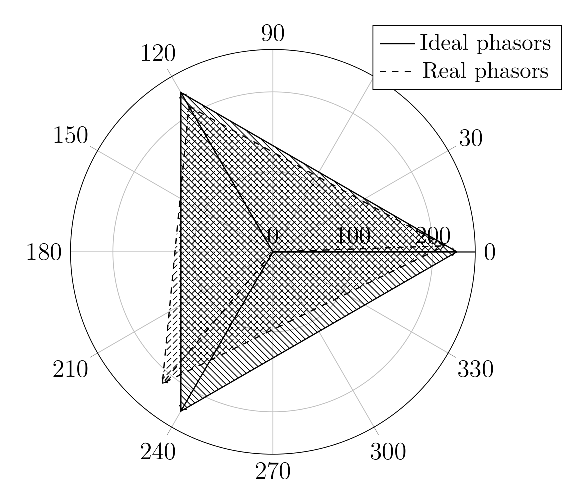
\includegraphics[scale=0.95]{Unblance_EPS_Pics/UnbalRedComp_JCP-figure1.eps}
           \caption{The triangles spanned by the ideal and the actual voltage phasors. The extent of voltage deviation on the network can be measured by the sum of areas where the two triangles are not overlapping.}
           \label{fig:threephase}
            \end{figure}

\section{The method's novelty compared to VUF}\label{VUB:sec:AdditionalContent}

When using a new norm for calculation and cost function it is reasonable to test it's usability against the prevalent or regulated method the voltage unbalance factor ($VUF$) defined by the International Electrotechnical Commission, as discussed in section \oldref{BASICUNB:sec:VUFCVUF}. In this case the geometrical norm's utility \ref{equ:geom} against the $VUF$ value shall be examined. \\
The geometrical norm was validated experimentally, by investigating the correlation between the regulated  and geometrical norms subjected to random, uniformly distributed unbalance on the voltage vector amplitude and phase values with $20$ V amplitude and $1/300\cdot\pi$ rad phase variance (Fig. \ref{fig:correlation}, and Fig. \ref{fig:side_correlation}).

            \begin{figure}[!ht]
           \centering
           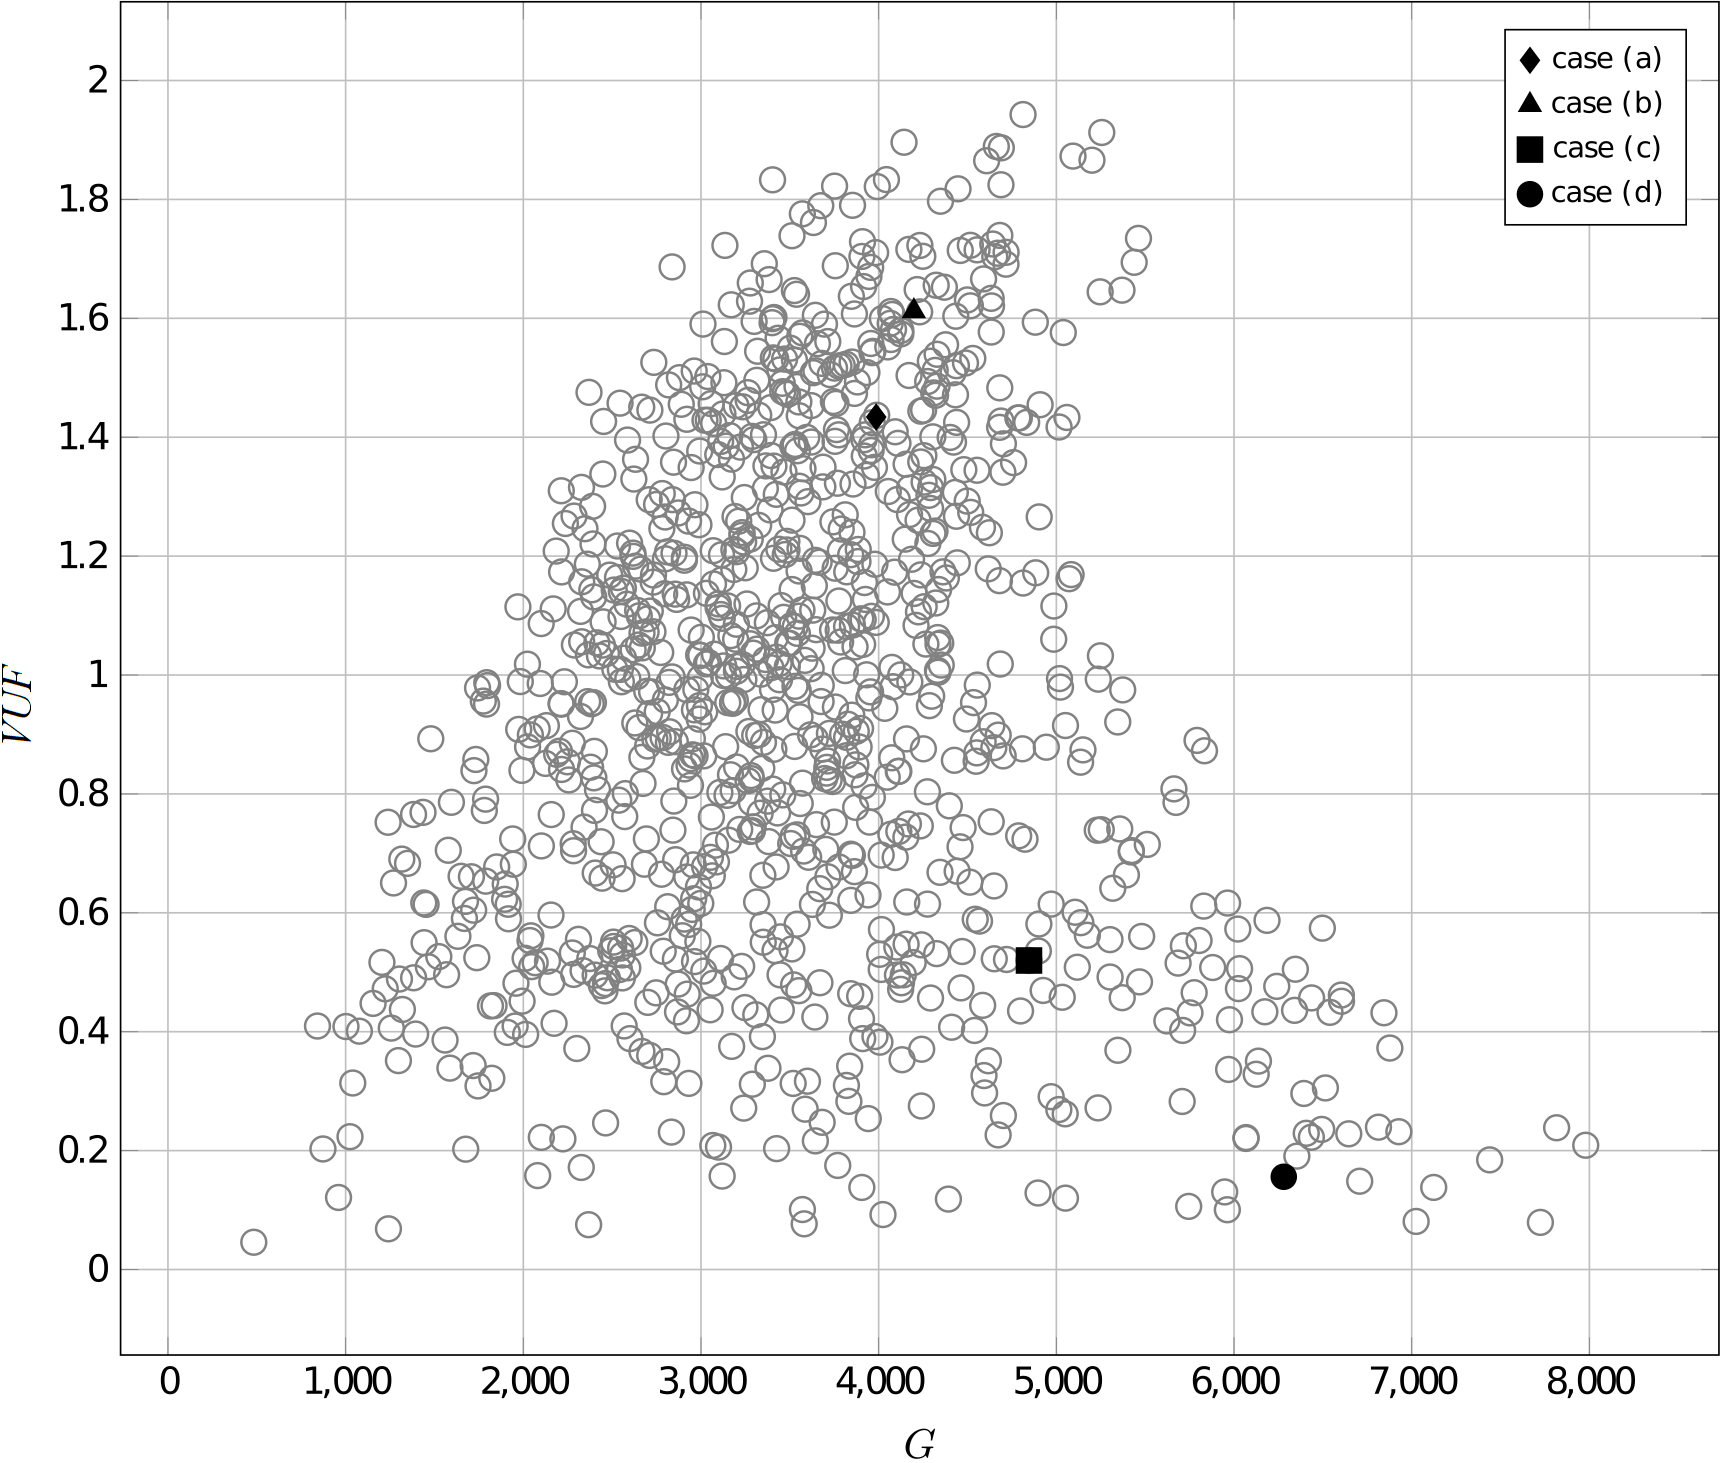
\includegraphics[width=\textwidth,scale=0.95]{Unblance_EPS_Pics/EPS_images/scatter.png}
           \caption{Correlation between the geometrical voltage unbalance indicator $G$ and the regulated voltage unbalance indicator $VUF$ using 1000 samples. In every iteration each three phase voltage vector's amplitude and phase values changed randomly, according to uniform distributions with $\pm20$ V amplitude and $\pm\frac{1}{3}\pi\cdot10^{-2}$ rad phase variance. It can be seen, that the geometric norm contains more information than the classical one. The  four asymmetry cases of Figure \ref{fig:cases} are denoted by black symbols on the picture. It is apparent, that in case (c), and (d) the G norm holds additional information than the $VUF$.}
           \label{fig:correlation}
            \end{figure}

            \begin{figure}[!ht]
           \centering
           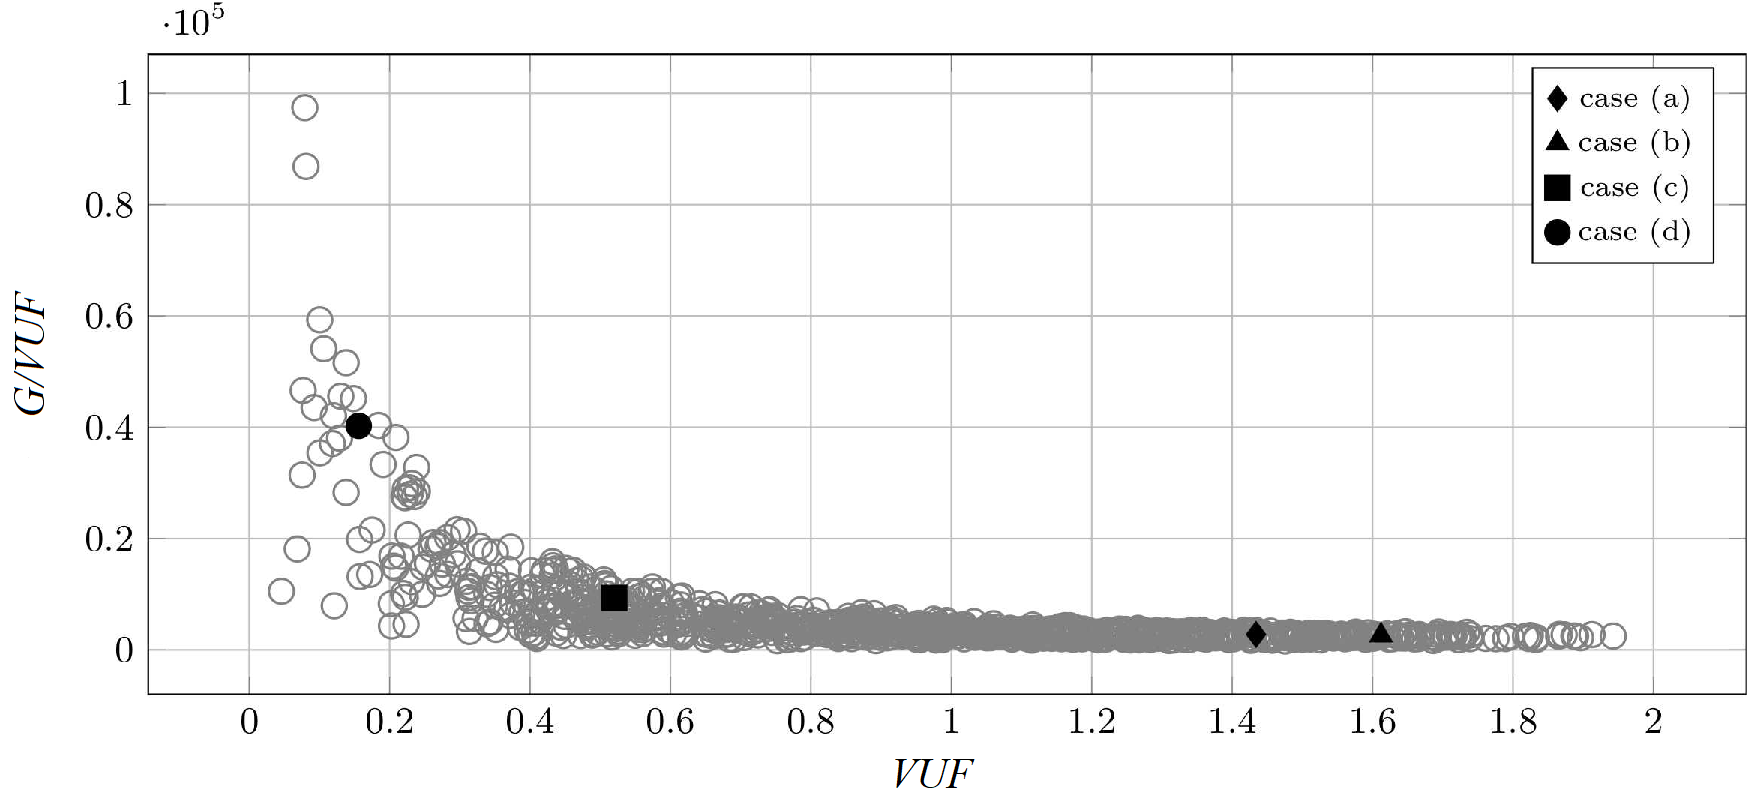
\includegraphics[width=\textwidth,scale=0.95]{Unblance_EPS_Pics/EPS_images/side_scatter.png}
           \caption{ Correlation between the regulated unbalance indicator and the fraction of geometrical and regulated indicator. It can be seen that there is a functional connection between the two values.}
           \label{fig:side_correlation}
            \end{figure}


            Although there is correlation between the two norm values in the general case, but for some situations the regular method indicates low, while geometrical norm still indicates high value.\\
            On Figure \ref{fig:cases_A} dominant phase deviation can be observed, while Figure \ref{fig:cases_B} shows amplitude deviation but with opposite direction. When there is such deviation on the grid both indicators present almost identical results. On \ref{fig:cases_C} there is still observable unbalance (two phase deviate stronger than the third in terms of amplitude), but the correlation is significantly lower. In the last case in the lowest correlation area, amplitude deviation is present, but the deviation direction is identical on all phases (balanced over-voltage or under-voltage, can be observed on Figure \ref{fig:cases_D}). The regular method indicates very low values. In this case other methods are utilised in parallel in terms of network diagnostics to detect the under-voltage phenomena.\cite{arn1997under-voltage}.


            \begin{figure}
                \centering
                \begin{subfigure}[b]{0.48\textwidth}
                    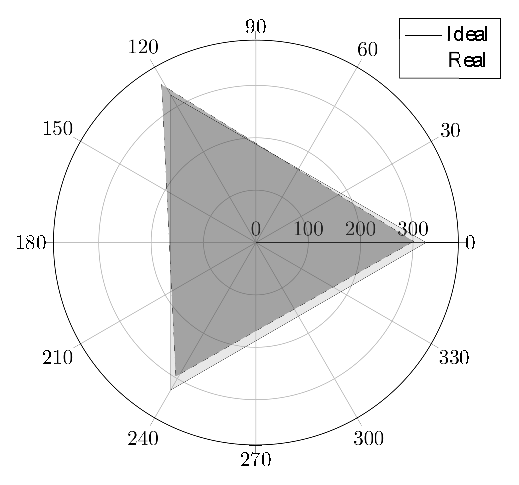
\includegraphics[width=\textwidth]{Unblance_EPS_Pics/EPS_images/rombus.eps}
                    \caption{\centering High correlation with phase deviation. The norm values are $G=3986$ and $VUF=1.434$.}
                    \label{fig:cases_A}
                \end{subfigure}
                ~ %add desired spacing between images, e. g. ~, \quad, \qquad, \hfill etc.
                  %(or a blank line to force the subfigure onto a new line)
                \begin{subfigure}[b]{0.48\textwidth}
                    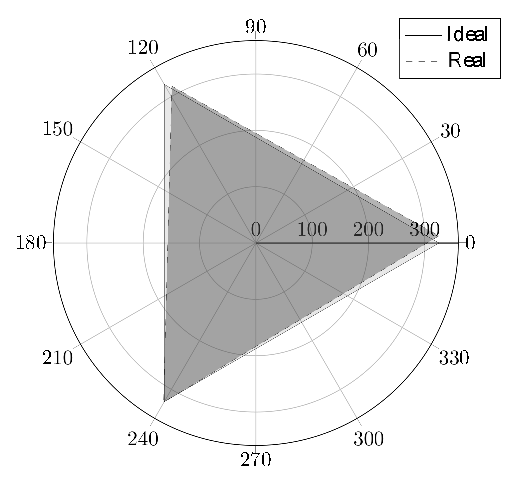
\includegraphics[width=\textwidth]{Unblance_EPS_Pics/EPS_images/triangle.eps}
                    \caption{\centering High correlation with opposed amplitude deviation. The norm values are $G=4198$ and $VUF=1.612$.}
                    \label{fig:cases_B}
                \end{subfigure}
                 %add desired spacing between images, e. g. ~, \quad, \qquad, \hfill etc.
                %(or a blank line to force the subfigure onto a new line)
                \begin{subfigure}[b]{0.48\textwidth}
                    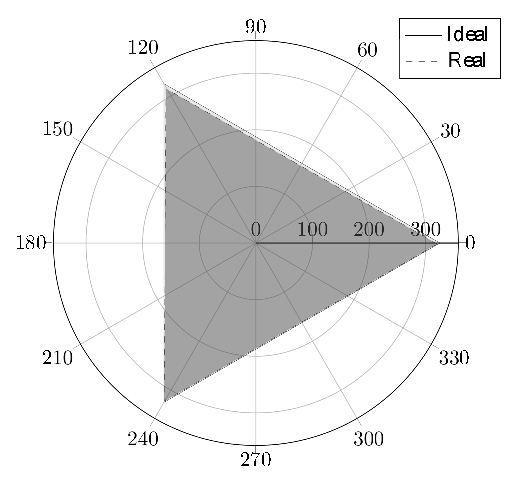
\includegraphics[width=\textwidth]{Unblance_EPS_Pics/EPS_images/square.eps}
                    \caption{Low correlation with opposed amplitude deviation. The norm values are $G=9322$ and $VUF=0.5198$.}
                    \label{fig:cases_C}
                \end{subfigure}
                ~
                \begin{subfigure}[b]{0.48\textwidth}
                    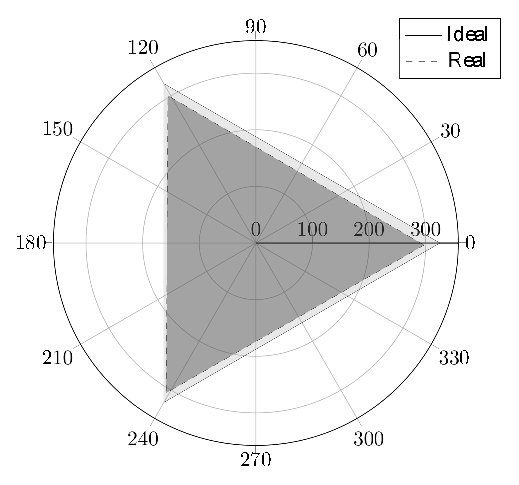
\includegraphics[width=\textwidth]{Unblance_EPS_Pics/EPS_images/circle.eps}
                    \caption{\centering Low correlation with uniform voltage drop. The norm values are $G=6280$ and $VUF=0.156$.}
                    \label{fig:cases_D}
                \end{subfigure}


                \caption{Four distinct cases of voltage triangles examining correlation between the regular $VUF$ and geometrical $G$ method.}\label{fig:cases}
            \end{figure}

To clarify this, the regular norm's calculation method needs to be investigated. The symmetrical component mutual impedance matrix on a three phase connection point is given by \ref{equ:mutual},

            \begin{equation}
                \begin{array}{rcl}
                       Z_s&=&\frac{1}{3}\begin{bmatrix} 1&1&1\\1&\upsilon&\upsilon^2\\1&\upsilon^2&\upsilon \end{bmatrix}\cdot
                                        \begin{bmatrix} Z_{aa}&Z_{ab}&Z_{ac}\\Z_{ba}&Z_{bb}&Z_{bc}\\Z_{ca}&Z_{cb}&Z_{cc} \end{bmatrix}\cdot
                                        \begin{bmatrix} 1&1&1\\1&\upsilon^2&\upsilon\\1&\upsilon\upsilon^2\end{bmatrix}=\\
                          &=&  \begin{bmatrix} Z_{00}&Z_{01}&Z_{02}\\Z_{10}&Z_{11}&Z_{12}\\Z_{20}&Z_{21}&Z_{22} \end{bmatrix},

                \end{array}
                \label{equ:mutual}
            \end{equation}

where $Z_s$ is the symmetrical component mutual impedance matrix, and $\upsilon=e^{j\frac{2}{3}\pi}$. If there are both negative and zero sequence symmetrical components present on the network, the dominant part of the voltage drop's negative and zero sequence can be calculated as follows \ref{equ:drop}.

            \begin{equation}
                \begin{array}{rcl}
                       \Delta U_2&\approx&Z_{21}I_1+Z_{22}I_2\\
                       \Delta U_0&\approx&Z_{01}I_1+Z_{00}I_0,
                \end{array}
                \label{equ:drop}
            \end{equation}

$\Delta U_0,\,\Delta U_1,\,\Delta U_2$ are the voltage drop's zero positive and negative sequence components, $I_0,\,I_1,\,I_2$ are the current's drop's zero positive and negative sequence components, and $Z_{00},Z_{01},\,Z_{21},\,Z_{22}$ are mutual impedances,  respectively. (If there is only positive and negative sequence present, then the right hand side's second term is zero.) As such, the indication of negative and zero sequence present the network calculates \ref{equ:factor}:

            \begin{equation}
                \begin{array}{rcl}
                       m_{21}&=&\mid\frac{Z_{21}}{Z_{11}}\mid\times100\\
                       m_{01}&=&\mid\frac{Z_{01}}{Z_{11}}\mid\times100,
                \end{array}
                \label{equ:factor}
            \end{equation}

where $m_{21}$ is the negative sequence factor which is identical to the $VUF$, and $m_{01}$ is the zero sequence factor.\\

\section{Summary}
At the previously described balanced over- or under-voltage case the positive sequence value is dominant, so the regular indicator will take considerably lower value. In other words, aside from indicating voltage unbalance, the geometrical method incorporates the balanced deviations as well. In a control design perspective, a general case, where notably highly unbalance values may appear, using $VUF$ as cost function could introduce hidden errors in control due error cancellation. Additionally the geometrical solution checks electrical asymmetry, i.e. the norm of a $\pm120$ degree rotated version of the ideal three-phase phasor is zero in the geometrical sense. Moreover, the geometrical norm is more sensitive for small scale unbalance, as opposed to the $VUF$. To summarize, the geometrical indicator a more suitable solution for a more general case indicator, and a good candidate for cost function in optimal control design. 